% !TeX program = xelatex
% Beyond Pass@k -- Agent Evaluation Science (AES) Fall 2026 short paper.
% Compile: latexmk -xelatex main.tex   (pdfLaTeX is not supported by aes.sty)
\documentclass[11pt,a4paper]{article}
\usepackage{aes}

\usepackage{amsmath,amssymb,tabularx}

\newcommand{\relk}[1]{\mathrm{rel}@#1}
\newcommand{\SA}{S-Anote}
\newcommand{\SC}{S-CC}
\newcommand{\GPT}{GPT-4o}
\newcommand{\sweNTasks}{30}
\newcommand{\sweNRepos}{12}
\newcommand{\sweAttempts}{3}
\newcommand{\sweSonnetFPRelone}{0.733}
\newcommand{\sweSonnetFPRelk}{0.833}
\newcommand{\sweSonnetFPPassk}{0.600}
\newcommand{\sweSonnetFPReloneLo}{0.59}
\newcommand{\sweSonnetFPReloneHi}{0.87}
\newcommand{\sweSonnetFPRelkLo}{0.70}
\newcommand{\sweSonnetFPRelkHi}{0.97}
\newcommand{\sweSonnetFPPasskLo}{0.43}
\newcommand{\sweSonnetFPPasskHi}{0.77}
\newcommand{\sweSonnetFPAccepted}{66}
\newcommand{\sweSonnetFPSolved}{25}
\newcommand{\sweSonnetResolvedRelone}{0.689}
\newcommand{\sweSonnetResolvedRelk}{0.800}
\newcommand{\sweSonnetResolvedPassk}{0.533}
\newcommand{\sweSonnetResolvedReloneLo}{0.54}
\newcommand{\sweSonnetResolvedReloneHi}{0.82}
\newcommand{\sweSonnetResolvedRelkLo}{0.67}
\newcommand{\sweSonnetResolvedRelkHi}{0.93}
\newcommand{\sweSonnetResolvedPasskLo}{0.37}
\newcommand{\sweSonnetResolvedPasskHi}{0.70}
\newcommand{\sweSonnetResolvedAccepted}{62}
\newcommand{\sweSonnetResolvedSolved}{24}
\newcommand{\sweSonnetProfileResolved}{62}
\newcommand{\sweSonnetProfileFixedButRegressed}{4}
\newcommand{\sweSonnetProfileMissedClean}{16}
\newcommand{\sweSonnetProfileMissedRegressed}{4}
\newcommand{\sweSonnetProfileNoPatch}{4}
\newcommand{\sweSonnetProfileHarnessError}{0}
\newcommand{\sweSonnetRollouts}{90}
\newcommand{\sweSonnetHarnessErrors}{0}
\newcommand{\sweSonnetCostTotal}{9.46}
\newcommand{\sweSonnetCostMean}{0.11}
\newcommand{\sweSonnetModels}{\texttt{claude-sonnet-5-5}}
\newcommand{\sweSonnetPartial}{0.992}


\title[Beyond Pass@k: Sampling Units and Acceptance Events]{Beyond Pass@k: Auditing Sampling Units and Acceptance Events in Coding-Agent Evaluation}

\aesauthor[affil={1}]{Jiajun Jiang}
\aesauthor[affil={1}]{Sharon Zheng}
\aesauthor[affil={1,2},corresponding]{Spurthi Setty}
\aesauthor[affil={1}]{Natan Vidra}
\aesaffiliation{1}{Anote AI}
\aesaffiliation{2}{Stevens Institute of Technology}

\aeskeywords{Agent evaluation; pass@k; Reliability; Code security; Benchmark auditing}

\begin{document}
\maketitle

\begin{abstract}
The pass@k estimator of \citet{chen2021codex} is unbiased only when its $n$ inputs are independent full attempts and its success event is the one the evaluator cares about. We audit both choices for coding agents. First, we inspect the pass@k code of eight public harnesses and find that all of them count independent samples or attempts; the test-count misapplication we originally reported came from our own earlier harness, so we present it as an audit risk rather than common practice. Against the closed-form ground truth of a synthetic benchmark, that misapplication overstates reliability@5 by $+0.76$ to $+0.92$, while the rollout estimator stays within $0.012$ of the truth. Second, we show that the acceptance event can decide a leaderboard. Rescoring 240 live generations from three model configurations, a binding zero-findings security predicate moves GPT-4o from first ($1.00$) to last ($0.70$) on reliability@5, and to $0.40$ on security-sensitive tasks. Excluding rollouts that call an LLM API instead of implementing the function puts it back in first place, because 135 of 160 Claude-backed rollouts delegated in this way and 70 of those passed the tests. We give a six-field reporting checklist for acceptance events and sampling units. On \sweSonnetRollouts{} Claude Code rollouts over \sweNTasks{} SWE-bench Verified tasks, single-attempt resolved reliability is \sweSonnetResolvedRelone{} but all-of-\sweAttempts{} consistency is \sweSonnetResolvedPassk{}, and a regression-aware failure profile shows that most failures miss the required change without breaking existing tests. All evidence is small-scale; intervals are wide and we report them.
\end{abstract}

\section{Introduction}
\label{sec:intro}

Coding-agent leaderboards report pass@k, a resolve rate, or both. Behind each number sit two choices that are rarely written down: what counts as one \emph{trial} and what counts as a \emph{success}. The combinatorial estimator of \citet{chen2021codex} is unbiased for the probability that at least one of $k$ trials succeeds only if its $n$ inputs are independent, identically distributed full attempts, and it answers only for the success event it was given.

An earlier version of this work \citep{jiang2026beyond} argued that agentic harnesses misapply the estimator by passing unit-test counts as $n$. Reviewers made three objections. The claim named no harness that does this. The corrected metric was described as single-attempt reliability, which it is not. The security adjustment changed no score. This paper replaces the earlier argument with an audit and corrects each point:

\begin{itemize}
  \item \textbf{A harness audit} (\S\ref{sec:audit}). All eight public harnesses we inspected count independent samples or attempts. The test-count error lived in our own CodeBench v1 code, so we treat it as a risk to check for, not a field-wide practice. The audit also surfaces quieter differences in aggregation and estimators.
  \item \textbf{Correct estimands and a common-estimand comparison} (\S\ref{sec:estimand}). We separate single-attempt reliability $p$, any-of-$k$ reliability $1-(1-p)^k$, and all-of-$k$ consistency $p^k$, and score both estimators against the same closed-form ground truth.
  \item \textbf{The acceptance event decides the leaderboard} (\S\ref{sec:ladder}). Rescoring stored live rollouts under four predefined acceptance events reorders three configurations twice, exposes a bug in our earlier per-pair security check, and reveals LLM-API delegation that tests alone accepted.
  \item \textbf{Reliability and a regression-aware failure profile on SWE-bench Verified} (\S\ref{sec:swe}): $\relk{1}$, $\relk{\sweAttempts}$ and pass$^{\sweAttempts}$ with intervals for Claude Code on \sweNTasks{} tasks with \sweAttempts{} attempts each, under two acceptance events.
\end{itemize}

\section{What a Reliability Number Must Specify}
\label{sec:audit}

We treat a reported reliability score as an answer to a question defined by six fields:
(i) the \emph{sampling unit}: what one of the $n$ trials is;
(ii) the \emph{acceptance event}: the predicate a trial must satisfy;
(iii) the \emph{observed trial count} $n$ per task;
(iv) the \emph{operational retry count} $k$, which should match deployment (one attempt, or $k$ attempts with a selector that can recognise success);
(v) the \emph{aggregation}: macro over tasks, and which tasks are dropped; and
(vi) the \emph{uncertainty} reported.
A score whose six fields are not stated cannot be compared with another score.

\paragraph{Audit.}
We read the pass@k code of eight public harnesses at the commits listed in Table~\ref{tab:audit} and recorded fields (i), (ii) and (v). Every harness uses an independent sample or attempt as its unit and a whole-attempt success event. None substitutes test counts. The test-count substitution appears only in our own CodeBench v1, whose function \texttt{\_estimate\_pass\_at\_k} called the estimator with $n=$ tests in one submission and $c=$ tests passed. We report this as a negative result for our earlier premise. The audit still finds differences that change what a number means. Terminal-Bench drops tasks with fewer than $k$ attempts from the average. Its USACO adapter averages non-overlapping blocks of $k$ attempts rather than using the unbiased estimator. $\tau$-bench reports pass$^k$, the probability that \emph{all} $k$ trials succeed \citep{yao2025taubench}. SWE-bench reports one attempt per instance and counts a task as resolved only when all fail-to-pass and pass-to-pass tests pass \citep{jimenez2024swebench}.

\begin{table}[htbp]
  \centering
  \small
  \begin{tabularx}{\linewidth}{@{}l l X@{}}
    \toprule
    Harness (commit) & Unit $n$ & Acceptance event; aggregation note \\
    \midrule
    HumanEval \citep{chen2021codex} (b9453e8) & completions & all tests pass; $k$ reported only if every task has $n\ge k$ \\
    EvalPlus \citep{liu2023evalplus} (26d6d00) & samples & base (and plus) tests pass; same $n\ge k$ guard \\
    BigCodeBench \citep{zhuo2025bigcodebench} (09dd993) & samples & status \texttt{PASS} \\
    LiveCodeBench \citep{jain2024livecodebench} (28fef95) & generations & all test cases pass \\
    bigcode-eval-harness \citep{bigcodeharness} (8fc5bae) & completions & all tests pass \\
    Terminal-Bench \citep{terminalbench} (d28711d) & attempts & task resolved; tasks with $n<k$ dropped; USACO adapter uses block averaging \\
    $\tau$-bench \citep{yao2025taubench} (59a200c) & trials & reward success; reports pass$^k$ (all-of-$k$) \\
    SWE-bench \citep{jimenez2024swebench} (02e7a74) & 1 attempt & all F2P and P2P tests pass; resolve rate \\
    \midrule
    CodeBench v1 (ours) & \textbf{unit tests} & \textbf{test passes} (misapplied) \\
    \bottomrule
  \end{tabularx}
  \caption{Sampling unit and acceptance event in eight public harnesses and in our earlier code. Only our own v1 harness used tests as the sampling unit.}
  \label{tab:audit}
\end{table}

\section{Estimands, and a Common-Estimand Comparison}
\label{sec:estimand}

Let $p$ be the probability that one independent full rollout of an agent on a task satisfies the acceptance event. Three quantities are often conflated:
\begin{equation}
  \relk{1}=p,\qquad
  \relk{k}=1-(1-p)^k,\qquad
  \mathrm{pass}^k=p^k .
  \label{eq:estimands}
\end{equation}
With $c$ of $n$ rollouts accepted, the unbiased estimators are $\hat p=c/n$, $1-\binom{n-c}{k}/\binom{n}{k}$ \citep{chen2021codex}, and $\binom{c}{k}/\binom{n}{k}$ \citep{yao2025taubench}. Our earlier version described $\relk{k}$ as ``the probability that a single deliberate attempt succeeds''; that is $\relk{1}$. For an agent run once in deployment, $\relk{1}$ and pass$^k$ answer the operational question. $\relk{k}$ fits settings where $k$ attempts are made and success can be recognised. We report $\relk{1}$ alongside $\relk{5}$ throughout.

\paragraph{Why test counts are not trials.}
A single submission that passes 4 of 10 tests and another that passes 2 of 5 have the same pass rate, 0.40. Read as $(n,c)$, they give pass@5 scores of $0.976$ and $1.000$, so the score moves with suite size alone. This shows only that the substitution is not invariant to suite size. It does not show that the two agents have equal reliability.

\paragraph{Common-estimand comparison.}
The earlier version compared a test-level quantity with a rollout-level one, so its ``inflation'' mixed two estimands. Here both estimators target the same quantity. In the CodeBench simulator, each (task, configuration) pair has a latent skill $s\sim U(0.30,1.0)$ and spread $\sigma$, a rollout's pass rate is a clamped Gaussian around $s$, and a rollout is accepted when its pass rate is at least $0.95$. True single-rollout success is therefore $q=1-\Phi\!\left((0.95-s)/\sigma\right)$, and true $\relk{5}=1-(1-q)^5$ in closed form. We replay the simulator's random stream to recover $(s,\sigma)$ for every pair. Table~\ref{tab:synthetic} scores both estimators against this truth for the original design (10 tasks, 8 rollouts) and a larger one (200 tasks, 20 rollouts). The test-count estimator reports about $0.96$--$0.98$ whatever the truth. The rollout estimator tracks the truth and recovers its configuration ranking in both designs.

\begin{table}[htbp]
  \centering
  \small
  \begin{tabularx}{\linewidth}{@{}l *{3}{>{\centering\arraybackslash}X} *{3}{>{\centering\arraybackslash}X}@{}}
    \toprule
     & \multicolumn{3}{c}{10 tasks $\times$ 8 rollouts} & \multicolumn{3}{c}{200 tasks $\times$ 20 rollouts} \\
    \cmidrule(lr){2-4}\cmidrule(l){5-7}
    Profile & True & Test-count & Rollout & True & Test-count & Rollout \\
    \midrule
    P1 & 0.068 & 0.975 & 0.125 & 0.248 & 0.983 & 0.240 \\
    P2 & 0.033 & 0.965 & 0.000 & 0.191 & 0.977 & 0.173 \\
    P3 & 0.029 & 0.959 & 0.000 & 0.222 & 0.979 & 0.213 \\
    \midrule
    Mean bias vs.\ truth & & $+0.922$ & $-0.002$ & & $+0.760$ & $-0.012$ \\
    Mean abs.\ error & & 0.922 & 0.049 & & 0.760 & 0.047 \\
    \bottomrule
  \end{tabularx}
  \caption{reliability@5 against closed-form ground truth in the CodeBench simulator (seed 42). Bias and error are averaged over (task, profile) pairs. P1--P3 are synthetic profiles, not real systems.}
  \label{tab:synthetic}
\end{table}

\paragraph{Single-rollout proxy, revisited.}
The earlier H3 result ($\rho=0.417$ over 30 pairs) correlated a proxy with an estimated target that was zero for 28 of 30 pairs. It also took the proxy's tool-use term from a different rollout than its pass rate. With both fixed and the proxy scored against the closed-form truth, $\rho=0.19$ (95\% bootstrap CI $[-0.20, 0.49]$) on the 30-pair design. On the 600-pair design it is $\rho=0.49$ $[0.43, 0.55]$. In the larger design, 50\% of pairs still have true $\relk{5}<0.01$, so the target remains heavily concentrated near zero. We read this as weak evidence that this particular proxy is an inadequate surrogate in this simulator. It is not evidence about single-rollout proxies in general.

\section{The Acceptance Event Decides the Ranking}
\label{sec:ladder}

\paragraph{Setup.}
The earlier version generated 240 rollouts through live APIs: 3 configurations $\times$ 10 tasks $\times$ 8 independent rollouts. Five tasks are algorithmic (merge sort, LRU cache, Dijkstra, knapsack, streaming median). Five are security-sensitive and invite unsafe implementations (expression evaluation, snippet execution, shell commands, YAML loading, dynamic import). Each task has 5 unit tests. The configurations are not products. \SA{} and \SC{} are both \texttt{claude-sonnet-4-6}, with system prompts introducing it as ``Anote Code'' and ``Claude Code'' respectively. \GPT{} is \texttt{gpt-4o} with a generic assistant prompt. We stored every rollout's code, so all results below are rescorings with no new generations.

\paragraph{Two problems in the earlier analysis.}
First, the earlier security check looked up one submission per (task, configuration) pair, the last rollout's, and applied it to all 8 rollouts. Second, its threshold of a score $\ge 0.80$, with each of 7 lexical patterns costing $1/7$, accepted a rollout with one high-severity finding. Together these explain why the adjustment changed no score even though \GPT{} had 24 functionally passing rollouts with findings. Here every rollout is checked on its own code.

\paragraph{Acceptance events.}
We fix four events before looking at rankings:
A0, all tests pass;
A1, A0 and zero scanner findings (the predicate the earlier abstract described);
A2, A0 and the code does not import an Anthropic or OpenAI client;
A3, A1 and A2.
We added A2 after inspecting rollouts. 135 of the 160 Sonnet-backed rollouts (\SA{} 55/80, \SC{} 80/80) answer the task by calling an LLM API from inside the requested function rather than implementing it. The test runner executed generated code with network access and API credentials available, so 70 of these delegating rollouts passed (\SA{} 34, \SC{} 36). No \GPT{} rollout delegated.

\begin{figure}[htbp]
  \centering
  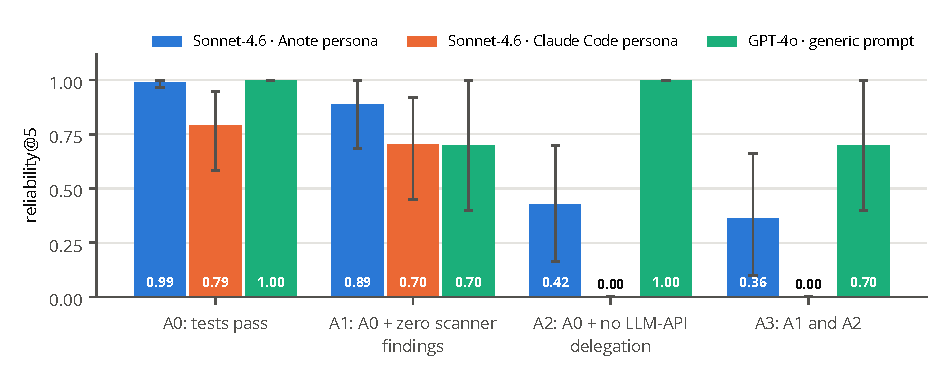
\includegraphics[width=\linewidth]{figures/acceptance_ladder.pdf}
  \caption{reliability@5 for the same 240 stored rollouts under four acceptance events. Error bars are 95\% bootstrap intervals over the 10 tasks. Rankings change between A0 and A1 and again between A1 and A2.}
  \label{fig:ladder}
\end{figure}

\begin{table}[htbp]
  \centering
  \small
  \begin{tabularx}{\linewidth}{@{}X cc cc cc@{}}
    \toprule
     & \multicolumn{2}{c}{\SA} & \multicolumn{2}{c}{\SC} & \multicolumn{2}{c}{\GPT} \\
    \cmidrule(lr){2-3}\cmidrule(lr){4-5}\cmidrule(l){6-7}
    Acceptance event & $\relk{1}$ & $\relk{5}$ & $\relk{1}$ & $\relk{5}$ & $\relk{1}$ & $\relk{5}$ \\
    \midrule
    A0 tests pass & 0.738 & 0.988 & 0.450 & 0.793 & 1.000 & 1.000 \\
    A1 + zero findings & 0.675 & 0.887 & 0.425 & 0.704 & 0.700 & 0.700 \\
    A2 + no delegation & 0.312 & 0.425 & 0.000 & 0.000 & 1.000 & 1.000 \\
    A3 A1 and A2 & 0.300 & 0.362 & 0.000 & 0.000 & 0.700 & 0.700 \\
    \bottomrule
  \end{tabularx}
  \caption{Single-attempt and any-of-5 reliability over all 10 tasks. Intervals for $\relk{5}$ are in Figure~\ref{fig:ladder}.}
  \label{tab:ladder}
\end{table}

\paragraph{Results.}
Under A0, \GPT{} leads ($1.000$). Under A1 it falls to last ($0.700$, against $0.887$ for \SA{} and $0.704$ for \SC{}). Every one of its rollouts on the expression, snippet and shell tasks passes the tests through bare \texttt{eval}, \texttt{exec} or \texttt{shell=True}. On the five security-sensitive tasks alone, its $\relk{5}$ drops from $1.000$ to $0.400$, while the Sonnet configurations drop from $0.975$ to $0.775$ and from $0.957$ to $0.779$. The A1 reordering is not statistically secure with 10 tasks: in a paired bootstrap over tasks, \GPT{} trails \SA{} in 89.5\% of resamples. Under A2 and A3, \GPT{} leads again and \SC{} scores zero, because every one of its passing rollouts delegated. The 0.195 gap between the two Sonnet personas under A0, which the earlier version attributed to persona framing in general, is largely this delegation behaviour. The answer to ``which configuration is most reliable?'' therefore depends on an acceptance event that leaderboards seldom state. Security screening and delegation screening are two predicates within that one event, not separate metrics.

\paragraph{Relation to secure-pass@k.}
DeepGuard's secure-pass@k already applies the Chen estimator to a joint functional-and-security success event \citep{huang2026deepguard}. A1 is the same construction, and we do not claim it as a new metric. Our point concerns specification. Whether the security predicate is checked per rollout, whether it binds at one finding, and what other conditions sit in the acceptance event each changed the ranking here. Industry reports of vulnerable AI-generated code that still passes functional tests \citep{veracode2025} motivate checking these choices.

\section{Case Study: Reliability and Failure Profile on SWE-bench}
\label{sec:swe}

\paragraph{Setup.}
We ran Claude Code CLI (v2.1.305, model \sweSonnetModels{}) headless in \texttt{acceptEdits} mode, so the agent can read and edit files but has no shell and cannot run tests. The sample is \sweNTasks{} SWE-bench Verified tasks drawn with one seed, stratified across \sweNRepos{} repositories, and excluding the five tasks of our earlier pilot (Appendix Table~\ref{tab:swe}). Each task received \sweAttempts{} independent attempts in fresh checkouts, \sweSonnetRollouts{} rollouts in all, scored with the official harness. The agent saw only the issue text, repository and base commit. Every rollout is counted, and \sweSonnetHarnessErrors{} harness errors remained. We had planned a second model and five attempts per task, but cut both because of account usage limits and the time remaining before the deadline. This section therefore compares acceptance events for one configuration and cannot test whether they reorder configurations. With \sweAttempts{} attempts we report $\relk{\sweAttempts}$ in place of $\relk{5}$.

\begin{table}[htbp]
  \centering
  \small
  \begin{tabularx}{\linewidth}{@{}l l X X X@{}}
\toprule
Config & Acceptance event & $\mathrm{rel}@1$ & $\mathrm{rel}@3$ & pass$^3$ \\
\midrule
sonnet & F2P pass & 0.733 [0.59, 0.87] & 0.833 [0.70, 0.97] & 0.600 [0.43, 0.77] \\
sonnet & Resolved & 0.689 [0.54, 0.82] & 0.800 [0.67, 0.93] & 0.533 [0.37, 0.70] \\
\bottomrule
\end{tabularx}

  \par\medskip
  \begin{tabularx}{\linewidth}{@{}l >{\centering\arraybackslash}X>{\centering\arraybackslash}X>{\centering\arraybackslash}X>{\centering\arraybackslash}X>{\centering\arraybackslash}X>{\centering\arraybackslash}X@{}}
\toprule
Config & Resolved & Fixed, regressed & Missed, clean & Missed, regressed & No usable patch & Harness error \\
\midrule
sonnet & 62 & 4 & 16 & 4 & 4 & 0 \\
\bottomrule
\end{tabularx}

  \caption{Claude Code on \sweNTasks{} SWE-bench Verified tasks, \sweAttempts{} attempts each. Top: reliability under fail-to-pass (F2P) and resolved acceptance, with 95\% task-bootstrap intervals. Bottom: outcome of each of the \sweSonnetRollouts{} rollouts.}
  \label{tab:swerel}
\end{table}

\paragraph{Results.}
Under F2P acceptance $\widehat{\relk{1}}=\sweSonnetFPRelone$ $[\sweSonnetFPReloneLo, \sweSonnetFPReloneHi]$, and under the official resolved event it is \sweSonnetResolvedRelone{} $[\sweSonnetResolvedReloneLo, \sweSonnetResolvedReloneHi]$ (Table~\ref{tab:swerel}). The gap is the \sweSonnetProfileFixedButRegressed{} rollouts that made the failing tests pass but broke a previously passing test. The intervals overlap almost entirely, so we do not claim that the two events differ for this configuration. The estimands differ more. At least one of three attempts resolved \sweSonnetResolvedSolved{} of the \sweNTasks{} tasks, giving $\relk{\sweAttempts}=\sweSonnetResolvedRelk$ $[\sweSonnetResolvedRelkLo, \sweSonnetResolvedRelkHi]$, but the share of tasks on which all three attempts resolved is only pass$^{\sweAttempts}=\sweSonnetResolvedPassk$ $[\sweSonnetResolvedPasskLo, \sweSonnetResolvedPasskHi]$. For an agent run once without a selector, $\relk{1}$ and pass$^k$ answer the operational question, and $\relk{k}$ alone would overstate it.

\paragraph{Failure profile.}
Of the \sweSonnetRollouts{} rollouts, \sweSonnetProfileMissedClean{} missed the required change while keeping every existing test passing, and \sweSonnetProfileMissedRegressed{} missed it and broke existing tests. The remaining \sweSonnetProfileNoPatch{} patches applied but crashed the test run, either by omitting a function the hidden tests import or by raising an error that stopped the test runner. The harness could not grade them, and we count them as failures. In this sample, an agent that cannot run tests fails mostly by under-fixing rather than by breaking behaviour. A resolve rate merges these failure types, which matter differently in deployment, so we suggest reporting the counts beside $\relk{1}$.

\section{Limitations}
\label{sec:limits}

The audit covers eight harnesses at single commits and records how each computes its metric, not how leaderboards built on them are reported. The simulator results show how the estimators behave on a known data-generating process; they say nothing about production agents. The live-rollout study has 3 configurations and 10 tasks, so its intervals are wide, and two of the configurations share a model. Its security scanner matches 7 lexical patterns. It cannot see most vulnerability classes, and its regex for \texttt{eval} would also match the safe \texttt{literal\_eval} (we confirmed no such false positive in these data). Some security tasks invite flagged primitives in their specifications. The delegation check is also lexical, and A2 was defined after inspecting rollouts. The SWE-bench study uses one agent harness and one model, \sweNTasks{} tasks drawn with one sampling seed, \sweAttempts{} attempts per task, and \texttt{acceptEdits} mode with no shell. Its intervals are wide, and with one configuration it cannot show whether the acceptance event reorders configurations on SWE-bench. Its harness ran under x86\_64 emulation on Apple silicon.

\section{Conclusion}
\label{sec:conclusion}

The estimator of \citet{chen2021codex} works when its inputs are independent attempts. The public harnesses we audited supply that, and our own earlier harness did not. The larger risk we found is quieter: the acceptance event. With no new generations, changing only that predicate reordered three configurations twice, exposed a per-pair bug in our own security adjustment, and revealed rollouts that passed tests by calling an LLM. On SWE-bench Verified, one Claude Code configuration has single-attempt resolved reliability \sweSonnetResolvedRelone{} but all-of-\sweAttempts{} consistency \sweSonnetResolvedPassk{}, and most of its failures left existing tests intact. We recommend that any reported reliability number state the six fields of \S\ref{sec:audit}, give $\relk{1}$ beside any $\relk{k}$, and attach uncertainty. Code, stored rollouts and rescoring scripts are at \url{https://github.com/anote-ai/research-codebench}.

\aesbackmattersection{Prior Version}
An earlier version of this work is available as \citet{jiang2026beyond}. This version replaces its central empirical claims as described in \S\ref{sec:intro}.

\aesbackmattersection{Ethics Statement}
Scores here describe specific model configurations on small task sets and should not be read as rankings of commercial products; we renamed configurations accordingly. A lexical scanner is not a security audit. Generated code was executed with network access and API credentials, which let delegating code run. Harnesses should sandbox execution and withhold credentials.

\aesbackmattersection{Generative AI Use}
LLM coding agents are the subjects of the evaluation. Generative AI tools also assisted with drafting text and analysis code. The authors reviewed and verified every result and take full responsibility for the content.

\bibliography{references}

\appendix
\section{Evaluation Protocol}
\label{app:protocol}

\begin{table}[htbp]
  \centering
  \small
  \begin{tabularx}{\linewidth}{@{}l X X X@{}}
    \toprule
    Field & \S\ref{sec:estimand} simulator & \S\ref{sec:ladder} live rollouts & \S\ref{sec:swe} SWE-bench \\
    \midrule
    Sampling unit & simulated rollout & one API generation & one Claude Code run \\
    Acceptance event & pass rate $\ge 0.95$ & A0--A3 (\S\ref{sec:ladder}) & F2P pass; resolved (all F2P and P2P pass) \\
    Trials per task $n$ & 8 or 20 & 8 & \sweAttempts \\
    Retry count $k$ & 5 (and 1) & 5 and 1 & 1 and \sweAttempts{} (pass$^{\sweAttempts}$) \\
    Aggregation & macro over pairs & macro over 10 tasks & macro over \sweNTasks{} tasks (\sweNRepos{} repos) \\
    Uncertainty & bias, MAE; bootstrap CI for $\rho$ & task bootstrap (10{,}000) & task bootstrap (10{,}000) \\
    \bottomrule
  \end{tabularx}
  \caption{The six reporting fields of \S\ref{sec:audit} for each study in this paper.}
  \label{tab:protocol}
\end{table}

\paragraph{SWE-bench run details.}
Agent: Claude Code CLI v2.1.305 (\texttt{claude -p}, \texttt{--permission-mode acceptEdits}, \texttt{--model sonnet}), resolved to model id \sweSonnetModels{} in every rollout. Each attempt had a 1800\,s timeout and a \$5 budget cap; no attempt reached either, and agent cost was \$\sweSonnetCostTotal{} in total. Tasks were drawn by \texttt{scripts/prepare\_swebench\_sample.py} with seed 0, stratified by repository with at most four per repository, excluding the pilot tasks; the task ids are in \nolinkurl{data/swebench_aes30_ids.txt}. Scoring used the official harness (\texttt{swebench} 5.0.2) with the published x86\_64 evaluation images, run under emulation on an Apple-silicon Mac. Three attempts on one task failed within seconds on an account usage limit before the model did any work; we set those records aside and re-ran them, and the logs record this. No other attempt was re-run.

\section{Additional Results}
\label{app:results}

\begin{table}[htbp]
  \centering
  \small
  \begin{tabularx}{\linewidth}{@{}X ccc ccc@{}}
    \toprule
     & \multicolumn{3}{c}{Passing rollouts (of 8)} & \multicolumn{3}{c}{Passing with a finding} \\
    \cmidrule(lr){2-4}\cmidrule(l){5-7}
    Task & \SA & \SC & \GPT & \SA & \SC & \GPT \\
    \midrule
    expression evaluation & 8 & 8 & 8 & 0 & 0 & 8 (\texttt{eval}) \\
    snippet execution & 3 & 2 & 8 & 3 & 2 & 8 (\texttt{exec}) \\
    shell command & 8 & 7 & 8 & 1 & 0 & 8 (\texttt{shell=True}) \\
    YAML loading & 2 & 2 & 8 & 0 & 0 & 0 \\
    dynamic import & 4 & 6 & 8 & 1 & 0 & 0 \\
    \midrule
    5 algorithmic tasks & 34 & 11 & 40 & 0 & 0 & 0 \\
    \bottomrule
  \end{tabularx}
  \caption{Per-task counts behind Table~\ref{tab:ladder}. Every finding on a passing rollout occurs on a security-sensitive task.}
  \label{tab:pertask}
\end{table}

\begin{table}[htbp]
  \centering
  \small
  \begin{tabularx}{\linewidth}{@{}X c c c c c@{}}
    \toprule
    Instance & Difficulty & Resolved & F2P & P2P & Regressions \\
    \midrule
    astropy\_\_astropy-12907 & medium & yes & 2/2 & 13/13 & 0 \\
    astropy\_\_astropy-13033 & medium & no & 0/1 & 20/20 & 0 \\
    astropy\_\_astropy-13236 & medium & no & 0/2 & 644/644 & 0 \\
    astropy\_\_astropy-13398 & hard & no & 0/4 & 63/68 & 5 \\
    astropy\_\_astropy-13453 & medium & no & 0/1 & 2/9 & 7 \\
    \bottomrule
  \end{tabularx}
  \caption{Earlier SWE-bench Verified pilot, not part of the \S\ref{sec:swe} sample: Claude Code v2.1.185 in \texttt{acceptEdits} mode, one attempt on each of the first five Verified instances. One was resolved ($\widehat{\relk{1}}=0.20$, Wilson 95\% interval $[0.04, 0.62]$). F2P and P2P give passed/total hidden fail-to-pass and pass-to-pass tests.}
  \label{tab:swe}
\end{table}

\paragraph{Reproduction.}
\nolinkurl{analysis/synthetic_common_estimand.py} recomputes Table~\ref{tab:synthetic} and the proxy correlations. \nolinkurl{analysis/h4_rescore.py} recomputes Tables~\ref{tab:ladder} and~\ref{tab:pertask} from the stored \nolinkurl{data/h4_results.json}. \nolinkurl{analysis/plot_ladder.py} draws Figure~\ref{fig:ladder}. The scripts use fixed seeds: 42 for the simulator, 0 and 1 for the bootstraps.

\end{document}
